\chapter{Introduction}

This chapter introduces the problem of real-time conversational avatars for Bangla, the motivation for the project, its objectives and methodology, and the outcome that was delivered.

\section{Project Overview}
Advances in speech recognition, large language models and speech synthesis have made voice assistants such as Alexa, Siri and Google Assistant part of everyday life. In parallel, audio-driven talking-head models can now generate a photorealistic face whose lips follow an arbitrary speech signal. Combining the two gives a \textit{conversational avatar}: an assistant that answers with a face as well as a voice. That is more engaging, and more accessible to people who rely on visual speech cues, than audio alone.

\noindent
Almost all of this technology is built for English. The talking-head systems most widely used in research are trained on English video and evaluated on English benchmarks, and none of the open research systems we examined had been trained or evaluated on Bangla. Commercial cloud services have begun to offer Bangla voices for their avatars, but they are closed, run only in the cloud, are paid per minute, and publish no evaluation of how well their lips follow Bangla speech.

\noindent
This project builds an open alternative. The user speaks Bangla into a web browser; a conversational agent understands the request and replies in spoken Bangla; and a 2D avatar renders that reply with synchronised lip movement, all in real time. The avatar model, \textbf{Alapon}, is SyncTalk\_2D \cite{synctalk2d} adapted to Bangla and improved, and the whole avatar pipeline runs on a consumer laptop GPU.

\noindent
Building Alapon also produced a research result. The gap we closed in SyncTalk\_2D, a mouth that copies the input video instead of following the audio, turned out to be present in five of the six published lip-sync systems we tested, and invisible to the standard lip-sync metric. Those findings are being prepared as a journal paper (Section~\ref{sec:journal}).

\section{Motivation}

Existing AI communication systems handle Bangla poorly. They are configured around English, so Bangla speech is often transcribed into the wrong script or misunderstood, and most avatar systems are neither trained nor tested on Bangla lip movement. Audio-only assistants give no visual speech cues, which reduces engagement and excludes users who rely on lip reading. Most avatar systems also depend on large models running on datacentre GPUs, which makes them expensive and impossible to deploy where connectivity is limited.\\

\noindent
A real-time Bangla avatar that runs locally addresses these at once. A face that speaks the user's language is easier to engage with than a text interface, particularly for users who are not comfortable reading or typing. A model small enough to run on a consumer laptop can be deployed in schools, public offices and clinics that have neither reliable internet nor a GPU budget. The same system supports education, public-service guidance, customer support and assistive technology.\\

\noindent
For such a system, the lips must genuinely follow the speech. A mouth that moves when nobody is speaking, or that copies movement from the source video instead of the audio, defeats the purpose of a visible face. Checking this directly therefore became part of the project.

\section{Objectives}
The aim of the project is to build a real-time conversational avatar that speaks Bangla with accurate, audio-driven lip synchronisation. The specific objectives are:

\begin{enumerate}
    \item To build an end-to-end, real-time voice-to-voice-and-video conversational pipeline that understands and answers in Bangla.
    \item To select an avatar model that fits the project's requirements, adapt it to Bangla speech, and verify that its mouth motion is genuinely driven by the audio.
    \item To collect and prepare Bangla audiovisual data for training and evaluation.
    \item To keep the avatar within a real-time budget of 25 frames per second on consumer hardware.
    \item To evaluate the result objectively against published systems, and to report what that evaluation reveals about the systems and their metrics.
\end{enumerate}


\section{Methodology}

The project followed the sequence below; each stage fed the next.\\

\noindent
\textbf{Stage 1 -- Identifying the gap.} We reviewed audio-driven talking-head generation and similar applications (Chapter~2). None of the open research systems had been trained or evaluated on Bangla, and most needed GPUs far beyond a laptop.\\

\noindent
\textbf{Stage 2 -- Building the real-time system.} We first built the complete pipeline with an English-speaking agent. This separated the engineering problems of latency, streaming and audio--video synchronisation from the linguistic problems of Bangla, and confirmed that the architecture could hold the real-time budget. We then built the Bangla agent on Google Gemini in speech-to-speech mode, with transcription pinned to Bangla, turn detection retuned for Bangla speech rhythm, and a formal-register Bangla persona.\\

\noindent
\textbf{Stage 3 -- Selecting the avatar model.} We chose SyncTalk\_2D because it is small and fast enough to run on a 4~GB laptop GPU, and confirmed the choice by testing published lip-sync systems on the same Bangla clip (Section~\ref{sec:selection}).\\

\noindent
\textbf{Stage 4 -- Adapting the model to Bangla.} We trained SyncTalk\_2D on Bangla video, retrained its lip-sync expert on Bangla, and built a streaming version of its audio features for live use. We also tried a multilingual speech encoder (XLS-R), which did not work.\\

\noindent
\textbf{Stage 5 -- Finding and closing the model's gaps.} The trained avatar moved its mouth when the audio was silent. We traced this to the model's mouth mask, which left the jaw visible, so the model copied mouth movement from the video instead of listening to the audio. We found three further gaps in the model's design and training and addressed all four. The result is \textbf{Alapon}, which we evaluated on lip-sync, silence, reconstruction quality and individual Bangla sounds.\\

\noindent
\textbf{Stage 6 -- Checking the leak in other models.} We applied the same silence test to six published systems on the Bangla clip and on the public English dataset HDTF. Five of the six leaked too, and the standard lip-sync metric did not detect it. This became the basis of a journal paper, now in progress.\\

\noindent
\textbf{Stage 7 -- Completing the system.} Alapon was integrated into the live system, and its speed and response time were measured on the target laptop.

\begin{figure}[H]
    \centering
    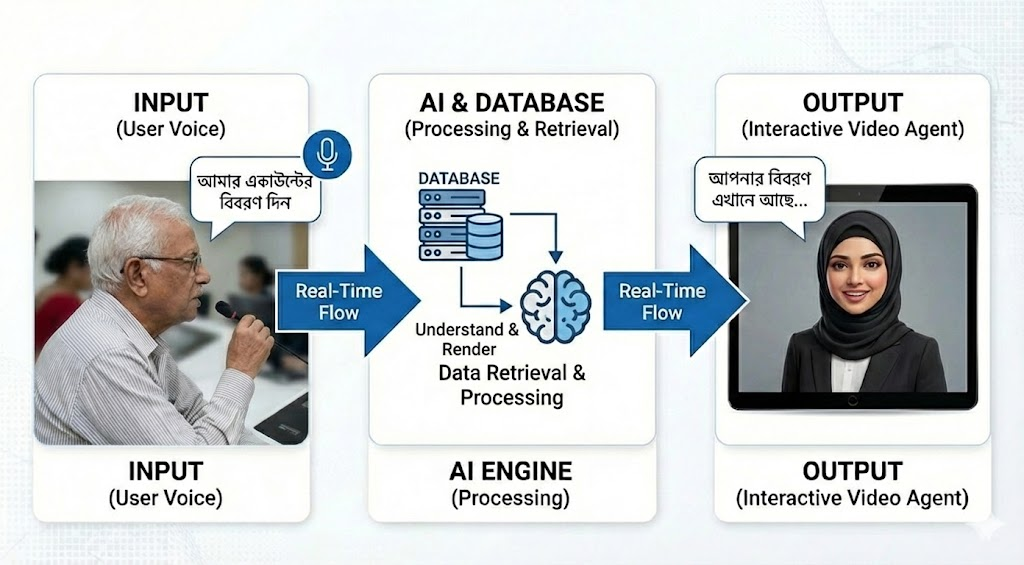
\includegraphics[width=0.8\textwidth]{Graphical_Abstract.jpg}
    \caption{Graphical Abstract}
    \label{fig: Graphical Abstract}
\end{figure}


\section{Project Outcome}

The project delivers a working real-time Bangla conversational avatar. Its main outcomes are:

\begin{itemize}
    \item A complete, running system: browser interface, real-time media layer, Bangla conversational agent and avatar rendering server.
    \item \textbf{Alapon}, a Bangla avatar model built on SyncTalk\_2D, 49~MB in size, rendering at 30 frames per second on a laptop RTX 3050 with 0.3~GB of GPU memory.
    \item Four gaps found and closed in the SyncTalk\_2D model. Covering the jaw stops the mouth moving during silence (41\% of frames $\rightarrow$ 0.1\%).
    \item A Bangla phoneme-to-viseme mapping and a Bangla sound-level evaluation, showing that Alapon's lips close on \bn{প}/\bn{ব}/\bn{ম} and open on \bn{আ}, including for six Bangla speakers it had never heard.
    \item A benchmark of six published systems on Bangla and English video with one scoring code, showing that five of the six leak on at least one dataset and that the standard lip-sync metric scores generated video above real video.
    \item A journal paper in preparation on these findings.
    \item A Bangla audiovisual corpus of 2.78 hours from 24 speakers, used as unseen test audio.
\end{itemize}

\noindent
The system is intended as a foundation for Bangla virtual tutors, public-service assistants, accessible interfaces and interactive media.


\section{Organization of the Report}

\begin{itemize}
    \item \textbf{Chapter 1 - Introduction} presents the problem, motivation, objectives, methodology and outcome of the project.

    \item \textbf{Chapter 2 - Background} covers the concepts needed for the rest of the report, reviews audio-driven talking-head generation and similar applications, and identifies the gap for Bangla.

    \item \textbf{Chapter 3 - Project Design} presents the requirements, the system architecture, how the avatar model was selected and adapted, the gaps found in it, and the project plan.

    \item \textbf{Chapter 4 - Implementation and Results} describes the implementation and reports the effect of closing the model's gaps, Bangla sound-level results, the comparison with published systems, the leakage found in them, and speed and response time.

    \item \textbf{Chapter 5 - Standards and Design Constraints} covers the engineering standards, design constraints, cost, and the complex engineering problem mapping.

    \item \textbf{Chapter 6 - Conclusion} summarises what was delivered against what was proposed, the limitations, the journal paper in progress, and future work.
\end{itemize}
